\documentclass{article}

\usepackage{arxiv}
\usepackage[T1]{fontenc}
\usepackage{amsmath,amssymb}
\usepackage{graphicx,booktabs,xcolor,colortbl,float,xspace}
\usepackage{microtype}
\usepackage[numbers,sort&compress]{natbib}
\usepackage{hyperref}

\graphicspath{{../../dblp_models/f_plot/output/pnas/}}
% generated by dblp_models/g_report/src/report.ipynb; refresh with make report
% FourYear = summed final four years; Career = whole-career supplement
% QQ excludes zero totals; means/Gini use all totals; Percent values omit the percent sign
\newcommand{\DBLPNComplete}{510}
\newcommand{\DBLPFourYearStart}{17}
\newcommand{\DBLPFourYearEnd}{20}
\newcommand{\ModelSeed}{63}
\newcommand{\DBLPFourYearQQRtwo}{0.975}
\newcommand{\DBLPFourYearMeanTotal}{28.127}
\newcommand{\DBLPFourYearGini}{0.467}
\newcommand{\DBLPFourYearNPositive}{500}
\newcommand{\DBLPFourYearNZero}{10}
\newcommand{\DBLPFourYearZeroPercent}{2.0}
\newcommand{\DBLPCareerQQRtwo}{0.992}
\newcommand{\DBLPCareerMeanTotal}{152.995}
\newcommand{\DBLPCareerGini}{0.360}
\newcommand{\DBLPCareerNPositive}{510}
\newcommand{\DBLPCareerNZero}{0}
\newcommand{\DBLPCareerZeroPercent}{0.0}
\newcommand{\DBLPRankInitialFinal}{0.187}
\newcommand{\DBLPRankLagThreeFinal}{0.653}
\newcommand{\DBLPRankLagFiveFinal}{0.583}
\newcommand{\DBLPFinalYearZeroPercent}{14.1}
\newcommand{\ARWFourFourYearQQRtwo}{0.991}
\newcommand{\ARWFourFourYearMeanTotal}{26.897}
\newcommand{\ARWFourFourYearGini}{0.318}
\newcommand{\ARWFourFourYearNPositive}{10000}
\newcommand{\ARWFourFourYearNZero}{0}
\newcommand{\ARWFourFourYearZeroPercent}{0.0}
\newcommand{\ARWFourCareerQQRtwo}{1.000}
\newcommand{\ARWFourCareerMeanTotal}{147.036}
\newcommand{\ARWFourCareerGini}{0.183}
\newcommand{\ARWFourCareerNPositive}{10000}
\newcommand{\ARWFourCareerNZero}{0}
\newcommand{\ARWFourCareerZeroPercent}{0.0}
\newcommand{\ARWFourRankInitialFinal}{0.002}
\newcommand{\ARWFourRankLagThreeFinal}{0.203}
\newcommand{\ARWFourRankLagFiveFinal}{0.077}
\newcommand{\ARWFourFinalYearZeroPercent}{0.0}
\newcommand{\GRWFourYearQQRtwo}{0.984}
\newcommand{\GRWFourYearMeanTotal}{41454.511}
\newcommand{\GRWFourYearGini}{0.992}
\newcommand{\GRWFourYearNPositive}{9825}
\newcommand{\GRWFourYearNZero}{175}
\newcommand{\GRWFourYearZeroPercent}{1.8}
\newcommand{\GRWCareerQQRtwo}{0.957}
\newcommand{\GRWCareerMeanTotal}{56998.145}
\newcommand{\GRWCareerGini}{0.985}
\newcommand{\GRWCareerNPositive}{10000}
\newcommand{\GRWCareerNZero}{0}
\newcommand{\GRWCareerZeroPercent}{0.0}
\newcommand{\GRWRankInitialFinal}{0.140}
\newcommand{\GRWRankLagThreeFinal}{0.833}
\newcommand{\GRWRankLagFiveFinal}{0.742}
\newcommand{\GRWFinalYearZeroPercent}{10.9}
\newcommand{\AROneFourYearQQRtwo}{0.992}
\newcommand{\AROneFourYearMeanTotal}{27.948}
\newcommand{\AROneFourYearGini}{0.507}
\newcommand{\AROneFourYearNPositive}{9999}
\newcommand{\AROneFourYearNZero}{1}
\newcommand{\AROneFourYearZeroPercent}{0.0}
\newcommand{\AROneCareerQQRtwo}{0.999}
\newcommand{\AROneCareerMeanTotal}{155.612}
\newcommand{\AROneCareerGini}{0.288}
\newcommand{\AROneCareerNPositive}{10000}
\newcommand{\AROneCareerNZero}{0}
\newcommand{\AROneCareerZeroPercent}{0.0}
\newcommand{\AROneRankInitialFinal}{0.001}
\newcommand{\AROneRankLagThreeFinal}{0.246}
\newcommand{\AROneRankLagFiveFinal}{0.100}
\newcommand{\AROneFinalYearZeroPercent}{2.5}
\newcommand{\HurdleAROneFourYearQQRtwo}{0.932}
\newcommand{\HurdleAROneFourYearMeanTotal}{25.129}
\newcommand{\HurdleAROneFourYearGini}{0.448}
\newcommand{\HurdleAROneFourYearNPositive}{9855}
\newcommand{\HurdleAROneFourYearNZero}{145}
\newcommand{\HurdleAROneFourYearZeroPercent}{1.5}
\newcommand{\HurdleAROneCareerQQRtwo}{0.987}
\newcommand{\HurdleAROneCareerMeanTotal}{135.411}
\newcommand{\HurdleAROneCareerGini}{0.255}
\newcommand{\HurdleAROneCareerNPositive}{10000}
\newcommand{\HurdleAROneCareerNZero}{0}
\newcommand{\HurdleAROneCareerZeroPercent}{0.0}
\newcommand{\HurdleAROneRankInitialFinal}{-0.012}
\newcommand{\HurdleAROneRankLagThreeFinal}{0.309}
\newcommand{\HurdleAROneRankLagFiveFinal}{0.136}
\newcommand{\HurdleAROneFinalYearZeroPercent}{15.7}
\newcommand{\ARSixFourYearQQRtwo}{0.936}
\newcommand{\ARSixFourYearMeanTotal}{23.469}
\newcommand{\ARSixFourYearGini}{0.442}
\newcommand{\ARSixFourYearNPositive}{9648}
\newcommand{\ARSixFourYearNZero}{352}
\newcommand{\ARSixFourYearZeroPercent}{3.5}
\newcommand{\ARSixCareerQQRtwo}{0.934}
\newcommand{\ARSixCareerMeanTotal}{136.980}
\newcommand{\ARSixCareerGini}{0.330}
\newcommand{\ARSixCareerNPositive}{9999}
\newcommand{\ARSixCareerNZero}{1}
\newcommand{\ARSixCareerZeroPercent}{0.0}
\newcommand{\ARSixRankInitialFinal}{0.129}
\newcommand{\ARSixRankLagThreeFinal}{0.592}
\newcommand{\ARSixRankLagFiveFinal}{0.531}
\newcommand{\ARSixFinalYearZeroPercent}{16.5}
\newcommand{\SEHurdleFourYearQQRtwo}{0.973}
\newcommand{\SEHurdleFourYearMeanTotal}{28.800}
\newcommand{\SEHurdleFourYearGini}{0.460}
\newcommand{\SEHurdleFourYearNPositive}{9741}
\newcommand{\SEHurdleFourYearNZero}{259}
\newcommand{\SEHurdleFourYearZeroPercent}{2.6}
\newcommand{\SEHurdleCareerQQRtwo}{0.967}
\newcommand{\SEHurdleCareerMeanTotal}{151.488}
\newcommand{\SEHurdleCareerGini}{0.341}
\newcommand{\SEHurdleCareerNPositive}{9998}
\newcommand{\SEHurdleCareerNZero}{2}
\newcommand{\SEHurdleCareerZeroPercent}{0.0}
\newcommand{\SEHurdleRankInitialFinal}{0.159}
\newcommand{\SEHurdleRankLagThreeFinal}{0.611}
\newcommand{\SEHurdleRankLagFiveFinal}{0.553}
\newcommand{\SEHurdleFinalYearZeroPercent}{14.3}
\newcommand{\DBLPQQRtwo}{\DBLPFourYearQQRtwo}
\newcommand{\ARWFourQQRtwo}{\ARWFourFourYearQQRtwo}
\newcommand{\GRWQQRtwo}{\GRWFourYearQQRtwo}
\newcommand{\AROneQQRtwo}{\AROneFourYearQQRtwo}
\newcommand{\HurdleAROneQQRtwo}{\HurdleAROneFourYearQQRtwo}
\newcommand{\ARSixQQRtwo}{\ARSixFourYearQQRtwo}
\newcommand{\SEHurdleQQRtwo}{\SEHurdleFourYearQQRtwo}
\newcommand{\GRWLognormalRtwo}{\GRWFourYearQQRtwo}


\title{Unequal scientific productivity emerges from stochastic temporal processes}
\renewcommand{\shorttitle}{Unequal scientific productivity}

\author{%
    Samantha Magid\textsuperscript{a,1} \quad
    Aanjaneya Kumar\textsuperscript{c} \quad
    Daniel B. Larremore\textsuperscript{d,c} \\
    Aaron Clauset\textsuperscript{d,c} \quad
    Sam Zhang\textsuperscript{a,b,c,d,1,2} \\[0.5em]
    \small\textsuperscript{a}Vermont Complex Systems Institute, University of Vermont, Burlington, VT 05405, USA. \\
    \small\textsuperscript{b}Department of Mathematics and Statistics, University of Vermont, Burlington, VT 05405, USA. \\
    \small\textsuperscript{c}Santa Fe Institute, Santa Fe, NM 87501, USA. \\
    \small\textsuperscript{d}Department of Computer Science, University of Colorado Boulder, Boulder, CO 80309, USA \\[0.4em]
    \small\textsuperscript{1}Equal contribution \quad
    \small\textsuperscript{2}Correspondence: \texttt{sam.zhang@uvm.edu}
}
\date{}

\begin{document}
\maketitle

\begin{abstract}
In 1957, William Shockley argued that the approximate lognormality of cumulative scientific productivity reflected the multiplicative effects of fixed differences in scientific ability. We tested this inference by comparing four stochastic models against longitudinal publication records. All four generated approximately lognormal publication totals without assigning researchers fixed differences in ability, yet they differed markedly in how well they reproduced individual career dynamics. A history-dependent hurdle model best reproduced the temporal patterns overall and most closely matched the empirical departures from lognormality. These results show that stochastic career dynamics can generate substantial inequality in publication output and that approximate lognormality alone cannot identify its sources.
\end{abstract}

\keywords{Scientific productivity \and science of science \and stochastic processes \and temporal dynamics}

\section{Introduction}
A central question in the study of scientific productivity is why publication output varies so widely across researchers. Research into this question began over a century ago with Lotka's Law of scientific productivity distribution~\cite{origins_of_productivity_frequency_law_lotka1926}. In the intervening century, the study of scientific productivity has attracted scientists from a wide array of fields, all aiming to turn their focus inwards. Notably, in 1957, Nobel Prize-winning physicist William Shockley observed that some scientists are dramatically more productive than others, and posited an influential explanation for why that is~\cite{product_of_factors_explains_lognormality_shockley1957}. Specifically, the rate of publications and patents produced by researchers in Shockley's dataset followed an approximately lognormal distribution, a heavy-tailed distribution where a minority of scientists were significantly more productive than the rest. Shockley sought to explain this through stable differences in individual cognitive and managerial talent.

\subsection*{Shockley's idea}\label{subsec:intro_shockley}
He gave the following framework to explain his observation. For sufficiently large $n$, assuming finite variance and negligible contributions from extreme fluctuations to the total variance, the sum of independently varying factors can be approximately normally distributed. Because a sum of logarithms is the logarithm of a product, Shockley concluded that the lognormally distributed publication counts $P$ were the product of $n$ independently varying aspects of scientific ability $F$:
\begin{equation}
P=\prod\nolimits_{i=1}^{n}F_i,
\qquad
F_1,\ldots,F_n\ \text{independent}
\ \Longrightarrow\ 
\log P=\sum\nolimits_{i=1}^{n}\log F_i \ 
\overset{\mathrm{approx}}{\sim} \
\mathcal{N}(\mu,\sigma^2), \quad F_i > 0
\label{eq:shockley_model}
\end{equation}
Shockley's contribution represented an influential proposal for an explanatory model of scientific productivity~\cite{shockley_in_modern_science_of_science_wang2021}. However, his model has several major shortcomings.

\subsection*{Atemporality}\label{subsec:intro_atemp}
Shockley's model describes variation in output across researchers over a fixed window. It leaves unspecified how each researcher's publications accumulate within that window. It lacks a temporal component, despite the fact that the accumulation of publications inherently occurs over time. Shockley's explanation therefore cannot explain any known temporal dynamics of scientific productivity. More fundamentally, explaining the distribution of accumulated output requires distinguishing the process of accumulation from the distribution it produces.
\subsection*{Non-identification}\label{subsec:intro_nonID}
Shockley infers a multiplicative structure from his observation that log productivity is approximately normally distributed. However, normality after taking logarithms does not establish that the underlying contributions combined multiplicatively: a lognormal distribution can also arise as a \emph{sum} of independent nonnegative random variables~\cite{thorinInfiniteDivisibilityLognormal1977}. Further, while cumulative lognormality can arise through multiplying components, that alone provides no basis for preferring his interpretation of those components as facets of scientific `ability' above anything else. 

\subsection*{Ideology of intrinsic human differences}\label{subsec:intro_eugenics}
Shockley, who would go on to gain notoriety for his advocacy of eugenicist beliefs, believed in the central importance of intelligence and other stable individual traits. He believed that scientific ability is generated by intelligence, and that intelligence is determined by immutable race and genetics, which intervention cannot meaningfully remediate~\cite{shockley_lectures_on_eugenics_and_research_taboos1967, shockley_public_hereditarian_and_eugenic_views1965, shockley_later_self_explanation_of_hereditarian_views1980}. Shockley's interpretation of the lognormal fit was consistent with these commitments. 

\subsection*{From publication totals to career trajectories}\label{subsec:intro_tots-to-trajs}
Later work has taken up both Shockley's observation of highly skewed output and his proposed explanation for it~\cite{called_shockley_elegant,shockley_in_modern_science_of_science_wang2021}. The inference at its core deserves closer scrutiny: what, if anything, does the shape of the productivity distribution tell us about fixed differences in scientific ability?

Zhang et al.~\cite{random_walk_reproduces_productivity_trajectories_zhang2026}
showed that a random walk fitted to annual publication histories can
generate approximately lognormal cumulative output without assigning
researchers fixed differences in ability. They also found departures
from lognormality in the observed totals. We build on these findings
by comparing temporal models against two kinds of evidence: how
publication output changes over a career, and how cumulative output
departs from a lognormal distribution.

\section{Empirical targets and model diagnostics}\label{sec:empirical_constraints}
To design temporal models, we first undertook exploratory data analysis of longitudinal publication records for 2,086 computer science researchers in the dblp computer science bibliography (`dblp dataset'). 

\begin{figure}[b]
    \centering
    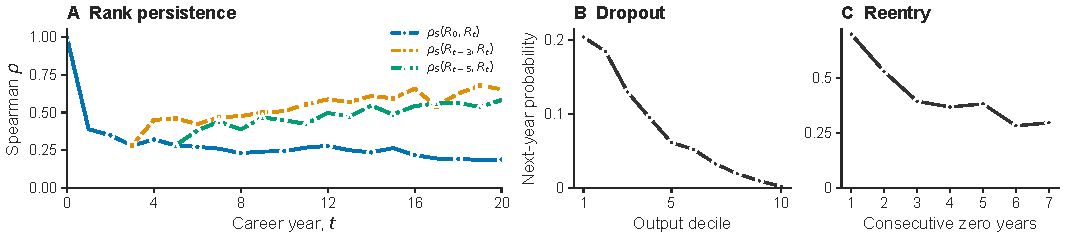
\includegraphics[width=\textwidth]{../../dblp_models/f_plot/output/pnas/pnas_dblp_temporal_wide.pdf}
    \caption{\textbf{Temporal patterns of publication in DBLP.}
    (A) Spearman correlations with year 0 ranks decline, while correlations at three- and five-year lags generally increase.
    (B) Among researchers who published in a given year, the probability of zero output the following year declines across current output deciles.
    (C) The probability of publishing the following year generally declines with the number of consecutive years of zero output.}\label{fig:dblp-rank-mixing}
\end{figure}

We identified three temporal patterns in DBLP publication histories (Fig.~\ref{fig:dblp-rank-mixing}). Annual publication ranks became less aligned with career-year 0 ranks as careers progressed, while rank correlations at fixed three- and five-year lags generally strengthened. Among researchers who published in a given year, those with higher output were less likely to record zero output the following year. Among researchers with zero output, the probability of publishing the following year generally fell as the inactive spell lengthened. These patterns give temporal models of productivity three targets beyond the distribution of cumulative output that motivated Shockley's account.

We compared simulated and observed productivity using distributional and
temporal diagnostics. For publication totals in career years 17--20,
matching the length of Shockley's observation window, we report the
median, mean, standard deviation, and Gini coefficient, and assess
lognormality among positive totals using QQ $R^2$. We quantify agreement
in annual output using the Wasserstein-1 distance between simulated and
observed distributions at each career year. We average these distances
($\bar{W}_1$) over years 0--20 and also summarize them within the career
stages identified by Zhang et al.~\cite{random_walk_reproduces_productivity_trajectories_zhang2026}.
For each of the two rank-persistence curves (fixed year~0 and fixed
five-year lag), we report the Spearman correlation at endpoint year~20
and the OLS slope over endpoint years 17--20. We summarize agreement
with the dropout and reentry patterns illustrated in
Fig.~\ref{fig:dblp-rank-mixing}B--C using RMSE in percentage points.
Dropout errors are weighted by the observed number of active
researcher-years in each output bin. Reentry errors are weighted by
the observed number at risk at each duration, using durations with
at least 20 observed cases at risk.

\begin{table}[t]
    \centering
    \caption{\textbf{Comparison of observed and simulated productivity.}
    The shaded row contains empirical dblp values. Slopes are changes in
    Spearman $\rho$ per career year, and RMSE is in percentage points (pp). Dashes indicate comparisons that use dblp as the reference.
    See~\ref{sec:empirical_constraints} for metric definitions.}\label{tab:model-comparison}
	\resizebox{\linewidth}{!}{%
		\begin{tabular}{@{}lrrrrrrrrrrrr@{}}
        \toprule
        & \multicolumn{5}{c}{Final four years (17--20)}
        & & \multicolumn{4}{c}{Rank persistence} & \multicolumn{2}{c}{RMSE (pp)} \\
        \cmidrule(lr){2-6}\cmidrule(lr){8-11}
        \cmidrule(l){12-13}
        Model & QQ $R^2$ & Med. & Mean & SD & Gini
        & $\bar{W}_1$ & $\rho_S(R_0, R_{20})$ & Slope & $\rho_S(R_{15}, R_{20})$ & Slope & Dropout & Reentry \\
        \midrule
        \rowcolor{gray!12}
        \textit{dblp}
        & \DBLPFourYearQQRtwo & \DBLPFourYearMedianTotal
        & \DBLPFourYearMeanTotal & \DBLPFourYearSDTotal
        & \DBLPFourYearGini & \textemdash
        & \DBLPRankInitialFinal & \DBLPRankInitialFourYearSlope
        & \DBLPRankLagFiveFinal & \DBLPRankLagFiveFourYearSlope
        & \textemdash & \textemdash \\
        GRW
        & \GRWFourYearQQRtwo & \GRWFourYearMedianTotal
        & \GRWFourYearMeanTotal & \GRWFourYearSDTotal
        & \GRWFourYearGini & \GRWAnnualWassersteinMean
        & \GRWRankInitialFinal & \GRWRankInitialFourYearSlope
        & \GRWRankLagFiveFinal & \GRWRankLagFiveFourYearSlope
        & \GRWDropoutRMSEPoints & \GRWRestartHazardRMSEPoints \\
        AR(1)
        & \AROneFourYearQQRtwo & \AROneFourYearMedianTotal
        & \AROneFourYearMeanTotal & \AROneFourYearSDTotal
        & \AROneFourYearGini & \AROneAnnualWassersteinMean
        & \AROneRankInitialFinal & \AROneRankInitialFourYearSlope
        & \AROneRankLagFiveFinal & \AROneRankLagFiveFourYearSlope
        & \AROneDropoutRMSEPoints & \AROneRestartHazardRMSEPoints \\
        H-AR(1)
        & \HurdleAROneFourYearQQRtwo & \HurdleAROneFourYearMedianTotal
        & \HurdleAROneFourYearMeanTotal & \HurdleAROneFourYearSDTotal
        & \HurdleAROneFourYearGini & \HurdleAROneAnnualWassersteinMean
        & \HurdleAROneRankInitialFinal & \HurdleAROneRankInitialFourYearSlope
        & \HurdleAROneRankLagFiveFinal & \HurdleAROneRankLagFiveFourYearSlope
        & \HurdleAROneDropoutRMSEPoints & \HurdleAROneRestartHazardRMSEPoints \\
        HD-H
        & \SEHurdleFourYearQQRtwo & \SEHurdleFourYearMedianTotal
        & \SEHurdleFourYearMeanTotal & \SEHurdleFourYearSDTotal
        & \SEHurdleFourYearGini & \SEHurdleAnnualWassersteinMean
        & \SEHurdleRankInitialFinal & \SEHurdleRankInitialFourYearSlope
        & \SEHurdleRankLagFiveFinal & \SEHurdleRankLagFiveFourYearSlope
        & \SEHurdleDropoutRMSEPoints & \SEHurdleRestartHazardRMSEPoints \\
        \bottomrule
    \end{tabular}
	}
\end{table}

\section{Temporal models}\label{sec:model}

We developed and tested several models of scientific productivity. Each model was developed in response to observed shortcomings in preceding models. Our models were designed by drawing from the literature of external fields with similar mathematical abstractions, including control theory, econometrics, and biostatistics, as well as from mathematical intuition about the nature of scientific productivity over time. Each model is fitted and evaluated against the dblp dataset using the above constraints and targets. For brevity, our reporting of results will refer to Table~\ref{tab:model-comparison}.

For models with stage-varying parameters, we use the career
changepoints that Zhang et al.\ estimated from publication
trajectories in the same dataset. They noted that the resulting
stages broadly aligned with the typical timing of tenure review
and promotion to full professor~\cite{random_walk_reproduces_productivity_trajectories_zhang2026}.
We assign each transition from career year $t$ to $t+1$ to a stage
$s(t)$ based on its starting year.
\begin{equation}
	s(t) =
	\begin{cases}
	1, & 0 \le t \le 4,\\
	2, & 5 \le t \le 7,\\
	3, & 8 \le t \le 13,\\
	4, & 14 \le t \le 19.
\end{cases}\label{eq:stages}
\end{equation}
We fit a separate parameter vector $\theta_j$ for each stage $j$.
Thus, $\theta(t)=\theta_{s(t)}$ is constant within each stage and
can change at the changepoints. This lets us capture changes in
productivity dynamics across the career with fewer parameters
than a year-specific fit.

\subsection*{Geometric Random Walk}\label{subsec:model_GRW}
We began with a geometric random walk (GRW) with IID lognormal multipliers on offset productivity. Let $P_t$ denote annual publication output in career year $t$, and let $\epsilon=0.49$ keep the logarithm finite at zero. We estimated $\hat\mu$ and $\hat\sigma^2$ by maximum likelihood from the observed increments $\log(P_{t+1}+\epsilon)-\log(P_t+\epsilon)$, pooled across all 20 career-year transitions. We sampled $P_0$ from the empirical career-year~0 distribution.

\begin{equation}
P_{t+1}=\max\{0,(P_t+\epsilon)e^{\eta_t}-\epsilon\},\qquad
\eta_t\overset{\mathrm{iid}}{\sim}
\mathcal{N}(\hat\mu,\hat\sigma^2).
\label{eq:grw}
\end{equation}

The GRW generated approximately lognormal career totals, yet substantially misrepresented other empirical properties; four-year mean and standard deviation are catastrophically overestimated, while the four-year median is only overestimated by roughly double, indicative of an extremely overdispersed model; its simulated Gini was also roughly double the empirical value, and it overestimated fixed-distance rank correlation while underestimating fixed-point rank correlation.

Thus, reproducing approximate lognormality did not yield an adequate model of productivity. The GRW, then, provides a twofold counterexample to the uniqueness of Shockley's explanation: successive stochastic shocks can generate an approximately lognormal cumulative distribution without assigning researchers fixed differences in ability, and reproducing an approximately lognormal cumulative distribution identifies neither a specific nor a consistent model. This does not exclude contributions from individual traits or establish the GRW as a sufficient explanation; it demonstrates that distributional form alone cannot identify Shockley's proposed mechanism.

\subsection*{First-order autoregressive}\label{subsec_model_AR1}
In the GRW, away from the zero boundary, each shock has a permanent
effect on log-offset productivity. This corresponds to the
unit-persistence case ($\beta=1$) of a first-order autoregressive
model. To allow shocks to decay, we estimated the intercept and
autoregressive coefficient separately within each career stage.

Writing $Y_t=\log(P_t+\epsilon)$, we modeled the update before
clipping as
\begin{equation}
Y_{t+1}=\hat\alpha_{s(t)}+\hat\beta_{s(t)}Y_t+Z_t,
\qquad
Z_t\overset{\mathrm{ind.}}{\sim}
\mathcal{N}(0,\hat\sigma^2_{s(t)}).
\label{eq:ar1}
\end{equation}

Within a career stage, $\beta$ determines how much of a shock
carries into the next year, while $\sigma$ measures the size of
typical year-to-year shocks. The intercept $\alpha$ and persistence
$\beta$ jointly determine the implied long-run mean of the
unclipped process if the stage parameters were held fixed. In analyzing the model output and parameters, we observed an intriguing trend in the autoregressive coefficients $\alpha$ and $\beta$. 

\begin{figure}[H]
    \noindent
    \begin{minipage}[t]{0.55\linewidth}
        \vspace{0pt}
        \centering
        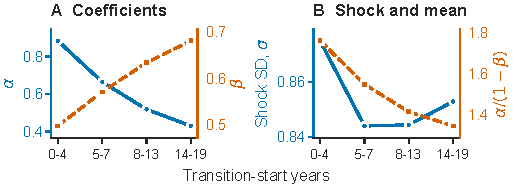
\includegraphics[width=\linewidth]{../../dblp_models/f_plot/output/pnas/pnas_dblp_ar1_stage_parameters.pdf}
        \caption{Fitted $\operatorname{AR}(1)$ parameters by career stage.}
        \label{fig:ar1-stage-parameters}
    \end{minipage}\hfill%
    \begin{minipage}[t]{0.42\linewidth}
        \vspace{0pt}
        Across career stages, $\beta$ increased while $\alpha$ declined
        (Fig.~\ref{fig:ar1-stage-parameters}). The decline in $\alpha$
        was large enough that the implied long-run mean,
        $\alpha/(1-\beta)$, fell on the log-offset scale. Shock
        variability was highest in the earliest stage and remained
        lower thereafter. Later-career shocks were thus modestly
        smaller and carried forward more strongly, a pattern
        consistent with the rise in fixed-lag rank correlations in
        Fig.~\ref{fig:dblp-rank-mixing}A. The fitted coefficients describe persistence in individual output. Rank persistence provides a separate check on the simulated careers.
    \end{minipage}
\end{figure}

The $\operatorname{AR}(1)$ retained approximate cumulative lognormality and brought the mean, median, and standard deviation of publication totals much closer to their empirical values, reducing $\bar{W}_1$ to less than two papers. Although its fixed-lag rank correlations increased over time, it substantially underpredicted both fixed-point and fixed-lag rank persistence. Its errors in dropout and reentry were also larger than those of the GRW, and it heavily underestimated the proportion of zero-publication streaks.

\subsection*{Hurdle autoregression}\label{subsec:model_hurdleAR}

To address AR(1)'s underestimation of zero-output years, we fitted a
hurdle autoregression (H-AR(1)). Following Baccini et al., we modeled
whether a researcher publishes in a given year (the extensive margin)
separately from how much they publish conditional on publishing (the
intensive margin)~\cite{bacciniCrossingHurdleDeterminants2014,longitudinal_zero_and_positive_outcomes_farewell2017}.

Let $A_t=\mathbf{1}\{P_t>0\}$ denote publication activity and let
$j=s(t)$ denote the stage of the transition from career year $t$ to
$t+1$. The probability of publishing in the next year is
\begin{equation}
\Pr(A_{t+1}=1\mid P_t)=
\begin{cases}
\hat r_j, & P_t=0,\\
1-\operatorname{logit}^{-1}\!\bigl(\hat d_j+\hat\gamma\log(P_t+\epsilon)\bigr),
    & P_t>0.
\end{cases}
\label{eq:har1-activity}
\end{equation}
We estimate the reentry probability $r_j$ and dropout intercept
$d_j$ separately by stage. The dropout slope $\gamma\leq 0$ is shared
across stages, allowing dropout probability to decline with current
output.

We set $P_{t+1}=0$ when $A_{t+1}=0$. Conditional on publication,
output follows
\begin{equation}
P_{t+1}\mid(A_{t+1}=1,P_t)\sim
\begin{cases}
\operatorname{Exponential}(\text{mean }\hat m_{\mathrm{re}}), & P_t=0,\\
\operatorname{LogNormal}(\hat\alpha_j+\hat\beta_j\log P_t,\hat\sigma_j^2),
    & P_t>0.
\end{cases}
\label{eq:har1-output}
\end{equation}
where the lognormal parameters are the mean and variance on the log
scale. We fit the AR(1) separately by stage using transitions between
two positive-output years. We estimate $m_{\mathrm{re}}$ from positive
outputs immediately following a zero-output year, pooling across stages.

H-AR(1) improved on AR(1) across most diagnostics, substantially
reducing reentry error and yielding the lowest dropout error of the
four models. Its cumulative totals remained approximately lognormal,
with the lowest QQ $R^2$ of the four models. Within each career stage,
its reentry probability was constant across inactivity durations,
whereas the observed probability generally declined as inactive spells
lengthened. By career year~20, simulated publication ranks still had
little association with initial ranks. These limitations motivated us
to incorporate earlier publication history into both margins.

\subsection*{History-dependent hurdle}\label{subsec:model_HD-H}

We retained the hurdle structure and allowed both margins to depend
on earlier publication history, yielding a history-dependent hurdle
model (HD-H). Let $x_t=\log(1+P_t)$ and $j=s(t)$. For the transition
from year $t$ to $t+1$, we summarize output before year $t$ by
\begin{equation}
H_0=0,\qquad
H_t=
\frac{\sum_{u=0}^{t-1}\hat\rho^{\,t-1-u}x_u}
     {\sum_{u=0}^{t-1}\hat\rho^{\,t-1-u}},
\quad t\geq 1.
\label{eq:hdh-history}
\end{equation}
This normalized exponential average encodes the inductive bias that
older output has less influence, with a single decay parameter
$\rho$ shared across stages and margins.

The extensive margin is a logistic regression for next-year
publication activity:
\begin{equation}
\Pr(A_{t+1}=1\mid P_t,H_t)=
\operatorname{logit}^{-1}\!\left(
\hat a_j+\hat b_j x_t+\hat c_j A_t+\hat d_j H_t
\right).
\label{eq:hdh-activity}
\end{equation}
We set $P_{t+1}=0$ when $A_{t+1}=0$. Conditional on publication,
we model log output by a linear regression with Gaussian shocks:
\begin{equation}
\log P_{t+1}\mid(A_{t+1}=1,P_t,H_t)
\sim
\mathcal{N}\!\left(
\hat\alpha_j+\hat\beta_j x_t+\hat\gamma_j(1-A_t)
+\hat\delta_j H_t,\,
\hat\sigma_j^2
\right).
\label{eq:hdh-output}
\end{equation}
The activity indicator $A_t=\mathbf{1}\{P_t>0\}$ distinguishes
currently active and inactive researchers in the extensive margin.
In the intensive margin, $1-A_t$ allows a separate intercept for
researchers returning to publication. We fit the coefficients
separately by career stage and select $\rho$ by cross-validation
with folds grouped by researcher.

\begin{table}[H]
    \centering
    \caption{Relative weight on earlier publication history in HD-H.
    Entries are the coefficient on $H_t$ divided by the coefficient
    on $x_t$ in the extensive ($\hat d_j/\hat b_j$) and intensive
    ($\hat\delta_j/\hat\beta_j$) margins.}
    \label{tab:seh-history-weight}
    \begin{tabular}{@{}lrr@{}}
        \toprule
        Transition-start years & Extensive & Intensive \\
        \midrule
        0--4   & \SEHurdleHistoryRatioExtensiveStageOne
               & \SEHurdleHistoryRatioIntensiveStageOne \\
        5--7   & \SEHurdleHistoryRatioExtensiveStageTwo
               & \SEHurdleHistoryRatioIntensiveStageTwo \\
        8--13  & \SEHurdleHistoryRatioExtensiveStageThree
               & \SEHurdleHistoryRatioIntensiveStageThree \\
        14--19 & \SEHurdleHistoryRatioExtensiveStageFour
               & \SEHurdleHistoryRatioIntensiveStageFour \\
        \bottomrule
    \end{tabular}
\end{table}

In the first career stage, earlier history $H_t$ received less than
half the weight per unit of most recent output $x_t$ in both margins.
After that stage, the two predictors received comparable weight per
unit (Table~\ref{tab:seh-history-weight}).

HD-H's simulated results were highly empirically consistent. It returned a $\bar{W}_1$ of just over half a paper, and closely matched mean, median, standard deviation, and Gini. It also most closely reproduced the slopes of both fixed-distance and fixed-point rank persistence, and the Spearman $\rho$ of the former, but fell short of GRW in the latter. HD-H also reduced reentry error by approximately 85\%, but its dropout error worsened slightly relative to H-AR(1).

In all 200 simulation runs, HD-H produced the lognormal QQ $R^2$ closest to the empirical value. Its QQ $R^2$ was below the empirical
value in 185 runs. To see whether this agreement extended to the
pattern of departures from lognormality, we compared QQ residuals
across percentiles. HD-H had the smallest RMS gap from the empirical
residual curve among the four models (Fig.~\ref{fig:qq-residuals}).

\begin{figure}[h]
    \centering
    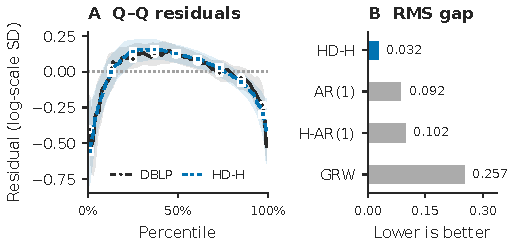
\includegraphics[width=\columnwidth]{../../dblp_models/f_plot/output/pnas/pnas_dblp_qq_residuals.pdf}
    \caption{\textbf{Departures from lognormality in final-four-year publication totals.}
    (A) QQ residuals for DBLP and HD-H among positive totals in career
    years 17--20. Shading shows pointwise 95\% bootstrap intervals.
    (B) RMS gap between each model's residual curve and DBLP's across
    the 1st through 99th percentiles.}\label{fig:qq-residuals}
\end{figure}


\section{Discussion}\label{sec:discussion}

William Shockley centered his explanation of scientific productivity around his observation of approximate cumulative lognormality, using a CLT-like argument to justify multiplicative accumulation, and his own eugenicist beliefs to infer traits of fixed ability. His work remains in currency due to his mathematical approach to explaining lognormality; with access to larger datasets and computing, we can confirm his observation of cumulative lognormality with greater rigor. However, as we have shown, simply reproducing cumulative lognormality, that is, returning a high QQ $R^2$, is insufficient to identify an otherwise-consistent model. There is only an 0.003 absolute difference in QQ $R^2$ between a model suggesting the mean output in the last four years is \GRWFourYearMeanTotal and one suggesting it is \AROneFourYearMeanTotal, against an empirical value of \DBLPFourYearMeanTotal; and in both cases, their $R^2$ is \emph{greater} than the empirical value. It seems instead that the specific way in which a model's CDF \emph{departs} from lognormality is identifying of broader consistency, with the RMS gap of HD-H being roughly a third of the next-closest model. All models and the empirical data are still highly lognormal ($\min \text{QQ} R^2 > 0.92$), and we are not suggesting that Shockley's observation of lognormality is inaccurate. However, his mathematical justification for his explanation centers about lognormality, and the fact that the best model is identified not by lognormality but by how it departs from lognormality weakens this point. 


\bibliographystyle{unsrtnat}
\bibliography{../paper/references}
\end{document}